% Drawing 148/01-12 -- folder 148, batch 01, archive page 17 (PDF page 18).
% Transcription: au milieu, à droite des sphères, un tétraèdre à l'encre verte et brune : deux arêtes opposées repassées en noir, l'arête cachée en pointillé vert ; un trait noir épais joint les milieux de deux arêtes opposées et deux traits verts épais le relient au sommet du haut et au sommet du bas ; du sommet du bas part une flèche vers la note de la marge droite.
% Kind: tetrahedron with a heavy H-shaped graph, arrow to the margin note. Method 2 (schematic redraw from the facsimile). Status: ok.
% Notes: Colour scan. Four vertices as heavy blots. The edges top-left, top-bottom and right-bottom thin, in brown (the right-bottom one doubled); the edges top-right and left-bottom heavy, ink over green. The hidden edge left-right is a row of eight brown dashes. In front, an H: a heavy ink stroke, slightly bowed, from a point of the top-left edge to a point of the right-bottom edge, and two heavy green strokes from the top vertex and from the bottom vertex down and up to it. Behind, a dotted H: from the left vertex a row of green dots up to a large green-black blot, three green dots from the start of the heavy stroke down to the same blot, a row of dark dots from it to a second blot, and from that one a row of green dots up to the right vertex; each dot is drawn where it stands. A thin ink arrow passes under the bottom vertex and points to the oblique note of the right margin (« ça fait 2^4 - 1 = 15 positions … »). This is the figure the note of the transcription calls « un grand tétraèdre tronqué, arêtes vertes et brunes, pointillés verts »: it is not truncated (the truncated one is the next figure, lower on the page). Redrawn 2026-11-12 (issue 128). 2026-11-13, Claude Opus 5.5, issue 147, overlay check: not compiled (no TeX in the session); the TikZ was rasterised by a local interpreter and laid over the 236 ppi scan rendered at 400 dpi. Redrawn on the ink: vertices and blots on their centres, edges fitted on their ink, the heavy stroke through points moved onto its ink, dots and dashes placed one by one; every stroke lies on its ink to within about one unit (the heavy strokes are wider on the page). Changed: the hidden edge is the row of brown dashes, not a green dotted line; the green and dark dots are drawn as a second, dotted H joining the left and right vertices through the two blots (the earlier redraw had the hidden edge green and two small dots); the heavy stroke and the heavy edges are moved onto their ink. Disagreement with the transcription: the hidden edge is in brown dashes; the green dots belong to the dotted second H (left vertex, blot, dark dots, blot, right vertex).
% Coordinates: 1 unit = 1 mm = 1/100 of the crop width, y downwards as on the crop (bbox in page fractions: [0.43, 0.245, 0.73, 0.405]).
% Redrawn by Claude (claude-fable-5-2), issue #128, 2026-11-12; not checked by a human; not compiled (no TeX in the session); overlay-checked on the scan by Claude Opus 5.5, issue #147, 2026-11-13, not compiled (no TeX in the session).
% Rights: reproduces part of the work -- behind RENDER_TRANSCRIPTS, never published by itself.
\documentclass[tikz,border=3pt]{standalone}
\usepackage{amsmath,amssymb}
\usetikzlibrary{patterns,arrows.meta}
\tikzset{pencil/.style={black!45}, struck/.style={black!35}, mpt/.style={circle,draw,inner sep=1.3pt}, pt/.style={circle,fill,inner sep=0.9pt}, opt/.style={circle,draw,fill=white,inner sep=1.1pt}, Rd/.style={red!75!black}, Gn/.style={green!45!black}, Br/.style={brown!70!black}}
\begin{document}
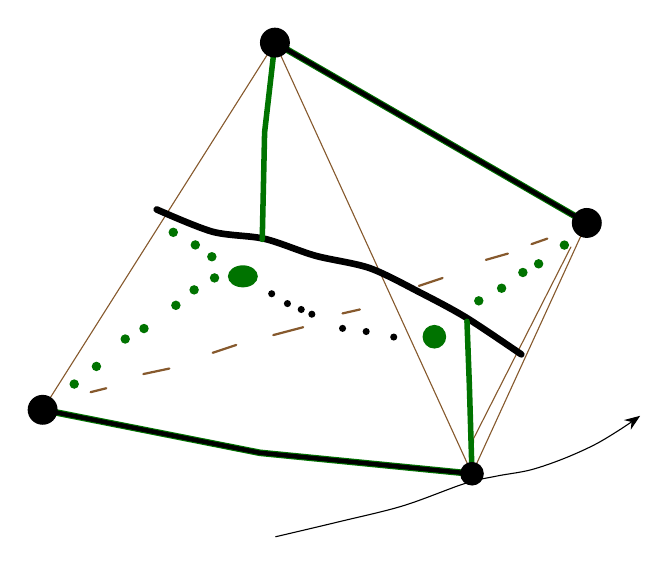
\begin{tikzpicture}[x=1mm,y=-1mm,line cap=round,line join=round,font=\small]
\coordinate (T) at (41.91,8.61);
\coordinate (R) at (81.52,31.51);
\coordinate (L) at (12.41,55.24);
\coordinate (B) at (66.94,63.36);
% thin brown edges (the right-bottom edge doubled)
\draw[Br] (T) -- (L);
\draw[Br] (T) -- (B);
\draw[Br] (R) -- (B);
\draw[Br] (79.5,34.56) -- (67.15,58.87) -- (B);
% heavy edges, ink over green
\draw[Gn,line width=2.4pt] (T) -- (R);
\draw[line width=1.6pt] (T) -- (R);
\draw[Gn,line width=2.4pt] (L) -- (40,60.7) -- (B);
\draw[line width=1.6pt] (L) -- (40,60.7) -- (B);
% the hidden edge left-right in brown dashes, as they stand
\draw[Br,thick] (18.5,53) -- (20.5,52.5);
\draw[Br,thick] (25.2,50.7) -- (28.5,50);
\draw[Br,thick] (34,48) -- (37,47);
\draw[Br,thick] (41.7,45.75) -- (45.5,44.75);
\draw[Br,thick] (50.5,43) -- (52.7,42.5);
\draw[Br,thick] (60.2,39.5) -- (63.2,38.5);
\draw[Br,thick] (68.7,36.2) -- (71.5,35.4);
\draw[Br,thick] (74.5,34.2) -- (76.5,33.5);
% the front H: heavy ink stroke from the top-left edge to the right-bottom edge, heavy green strokes from the top and the bottom vertex to it
\draw[line width=2.4pt] plot[smooth, tension=0.5] coordinates {(26.9,29.8) (33.97,32.62) (40.62,33.53) (47.04,35.67) (53.96,37.25) (60.49,40.42) (66.22,43.54) (73.2,48.2)};
\draw[Gn,line width=2pt] (T) -- (40.6,20) -- (40.3,33.6);
\draw[Gn,line width=2pt] (B) -- (66.6,52) -- (66.3,44);
% the dotted H behind: green dots from the left vertex and from the start of the heavy stroke to a blot, dark dots from it to a second blot, green dots from that one to the right vertex
\fill[Gn] (37.84,38.29) ellipse [x radius=1.9, y radius=1.4];
\fill[Gn] (62.16,45.96) circle [radius=1.5];
\foreach \p in {(16.42,51.97),(19.24,49.73),(22.9,46.25),(25.28,44.92),(29.33,41.97),(31.65,40.01),(34.24,38.49),(29,32.7),(31.8,34.3),(33.9,35.8),(78.67,34.32),(75.4,36.7),(73.4,37.8),(70.7,39.8),(67.8,41.4)} {\fill[Gn] \p circle [radius=0.6];}
\foreach \p in {(41.5,40.5),(43.5,41.75),(45.25,42.5),(46.6,43.1),(50.5,44.9),(53.5,45.3),(57,46)} {\fill \p circle [radius=0.45];}
\fill (T) circle [radius=1.9];
\fill (R) circle [radius=1.9];
\fill (L) circle [radius=1.9];
\fill (B) circle [radius=1.5];
% the ink arrow under the bottom vertex, to the oblique note of the right margin
\draw[-{Stealth[length=2mm]}] plot[smooth, tension=0.55] coordinates {(42.01,71.36) (50.04,69.46) (58.19,67.43) (66.02,64.6) (70.06,63.66) (74.35,62.88) (78.51,61.47) (82.52,59.67) (85.8,57.71) (88.3,56)};
\end{tikzpicture}
\end{document}
